%
% File acl2015.tex
%
% Contact: car@ir.hit.edu.cn, gdzhou@suda.edu.cn
%%
%% Based on the style files for ACL-2014, which were, in turn,
%% Based on the style files for ACL-2013, which were, in turn,
%% Based on the style files for ACL-2012, which were, in turn,
%% based on the style files for ACL-2011, which were, in turn, 
%% based on the style files for ACL-2010, which were, in turn, 
%% based on the style files for ACL-IJCNLP-2009, which were, in turn,
%% based on the style files for EACL-2009 and IJCNLP-2008...

%% Based on the style files for EACL 2006 by 
%%e.agirre@ehu.es or Sergi.Balari@uab.es
%% and that of ACL 08 by Joakim Nivre and Noah Smith

\documentclass[11pt]{article}
\usepackage{acl2015}
\usepackage{times}
\usepackage{url}
\usepackage{latexsym}
\usepackage{color, listings, graphicx, float, booktabs, multirow, outlines,changepage, fancybox, amsmath,enumitem, outlines}
\graphicspath{{./figures/}}

%\setlength\titlebox{5cm}

% You can expand the titlebox if you need extra space
% to show all the authors. Please do not make the titlebox
% smaller than 5cm (the original size); we will check this
% in the camera-ready version and ask you to change it back.

\definecolor{codegreen}{rgb}{0,0.6,0}
\definecolor{codegray}{rgb}{0.5,0.5,0.5}
\definecolor{codepurple}{rgb}{0.58,0,0.82}
\definecolor{backcolour}{rgb}{0.95,0.95,0.92}
 
\lstdefinestyle{mystyle}{
    backgroundcolor=\color{backcolour},   
    commentstyle=\color{codegreen},
    keywordstyle=\color{magenta},
    numberstyle=\tiny\color{codegray},
    stringstyle=\color{codepurple},
    basicstyle=\footnotesize,
    breakatwhitespace=false,         
    breaklines=true,                 
    captionpos=b,                    
    keepspaces=true,                 
    numbers=left,                    
    numbersep=5pt,                  
    showspaces=false,                
    showstringspaces=false,
    showtabs=false,                  
    tabsize=2
}
 
\lstset{style=mystyle}



\title{Instructions for ACL-2015 Proceedings}

\begin{document}
\begin{center}
	\textbf{\large{A Simple CUDA Neural Network}}\\
	Kyle Salitrik (kps168), Tomoki Takasawa (tmt5336)
\end{center}
\begin{abstract}
	This document covers the general purpose and workings of a neural network implemented to recognize handwritten digits. The MNIST dataset collected by the U.S. Government was used for all training and testing data. A mathematical background of neural networks is discussed followed by explicit discussion of the code implementation.
\end{abstract}

\section{Introduction and Purpose}
This program is designed to identify hand written numbers (0 ~ 9) by neural network digit classification technique. Generally, this technique requires enourmous amuont of run time. For training process, it calculates 5 matrix multiplications, 2 matrix subtractions, and 5 elemnt-wise vector operations. For verification, it requires 2 matrix multiplications and 2 element-wise operations for sigmoid function. In the case of all of the operations listed, the matrices and vectors are all densely populated. We decided to approach this problem by processing these operations in parallel on NVDIA's GPU processors. 

\section{Related Work}
Due to the age of neural networks, which were conceived in the 1940s, there is a large amount of documentation to reference. For the purposes of this paper, the first and second chapters of the online book Neural Networks and Deep Learning (NNDL) can be used a supplemental material (referenced at the end of the paper). Figures used in the Neural Network Structure and Forward Propagation sections were sourced from this book.

\section{Neural Network Background}
This portion of the document briefly covers the background on the mathematical methods employed for neural networks.

\subsection{Neural Network Structure}
The general purpose of the neural network is identifying handwritten digits 28x28 in size. An example of the handwritten data is shown below. This dataset, called MNIST, is commonly used to benchmark neural network performance. The handwriting samples were obtained by the U.S. National Institute of Standards and Technology (NIST) from both census workers and high school students. This data is divided into 50,000 training samples, 10,000 test samples, and 10,000 validation samples.

\begin{figure}[H]
	\centering
	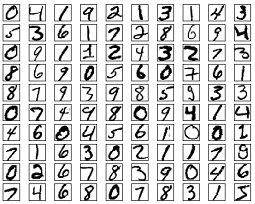
\includegraphics[width=.4\textwidth]{mnist_100_digits.png}
	\caption{MNIST Data, source: NNDL Book}
\end{figure}

Although it will be explained in the next section in detail, it is important to know that each neuron within the network will output a value between 0 and 1. This value is bound by what is called the activation function of the neuron. The input to the neural network was a matrix of 28x28 reshaped into a single column vector of size 784, with each neuron (vector element) representing a single pixel in the image. Initially the data is defined by a value of 0-127 for pixel intensity, but it is then bound to a value between 0 and 1 by simply dividing each element by 127. 

The hidden (or second) layer size of 128 neurons was arbitrarily chosen. While the objective was to train a simple neural network with only one hidden layer. A deep neural network may consist of a network with two or more hidden layers, typically each layer will reduce in size with each step forward in the network closer to the desired output layer size. These hidden layer sizes can be tuned (known as meta-parameters) in order to change the behavior of the network. The final (output) layer of the network consists of 10 neurons, with each neuron (0 through 9) representing the corresponding numerical digit. This format results in a vector similar to the following:
\begin{center}
	$[ 0, 0, 0, 1, 0, 0, 0, 0, 0, 0, 0 ]$\\
\end{center}
This representation is known as a 1-hot format, where the element that has a value of 1 indicates the corresponding digit as true. Referencing the above example, it represents the digit 3 (as element 3 has a value of 1). With regard to the output layer, the neuron with the highest value is chosen as the "answer" by the network. The structure for the neural network was as follows:
\begin{itemize}
	\item Layer 1 (input): 784 neurons
	\item Layer 2 (hidden layer): 128 neurons
	\item Layer 3 (output): 10 neurons
\end{itemize}


\subsection{Forward Propagation}
The behaivor of the neural network is defined by a function chosen by the network implementor. When a set of inputs are passed into a neuron layer (pictured below), each neuron in the layer computes its activation using this predetermined function. For the case of this assignment (and most simple neural networks), the sigmoid function was used. The sigmoid function helps us to bind the output from our neurons between 0 and 1 because we are looking for a (mostly) boolean answer: true or false for identifying a digit. This is where a significant portion of our computational cost comes from, as it includes a floating point exponential function, division and addition.
\begin{align}
	\sigma(z) & = \frac{1}{1 + e^{-z}} & \text{Sigmoid Function} 
\end{align}

\begin{figure}[H]
	\centering
	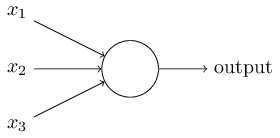
\includegraphics[scale=.5]{nn0.png}
	\caption{Neuron Diagram, source: NNDL Book}
\end{figure}

In our case, we use a densely connected neural network where every neuron in a layer is connected to every neuron in the following layer. It is useful to know that other types of layer relationships do exist such as sparsely connected layers, but are not explored here. These connections are defined by weight matrices where each element represents the connection from neuron A in layer L to neuron B in layer $L+1$.

\begin{figure}[H]
	\centering
	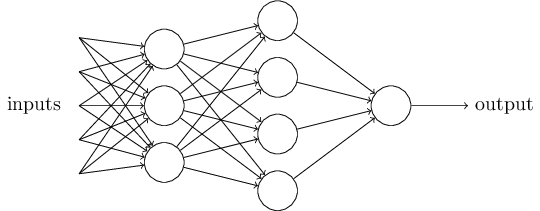
\includegraphics[width=.45\textwidth]{nn1.png}
	\caption{Network Diagram, source: NNDL Book}
\end{figure}

The majority of the computational costs arise from the vector-matrix multiplication between these dense weight matrices and the activations of the previous neurons. Each weight matrix is initalized to a random set of values and is adjusted during the final step (gradient descent) after each iteration through the network. In the following equations, $a^{(l)}$ represents the activation of layer $l$ and $\theta^{(l)}$ represents the weights between $a^{(l)}$ and $a^{(l+1)}$
 
To compute a full pass of forward propagation, we must compute the following equations:
\begin{align*}
	z^{(2)} & = a^{(1)}*\theta^{(1)T} \\
	a^{(2)} & = \sigma\{z^{(2)}\}     \\
	z^{(3)} & = a^{(2)}*\theta^{(2)T} \\
	a^{(3)} & = \sigma\{z^{(3)}\}     
\end{align*}

For our neural networks, the following are the weight matrix sizes:
\begin{itemize}
	\item Weight Matrix 1: 128x784 elements
	\item Weight Matrix 2: 10x128 elements
\end{itemize}

At this point, the forward propagation has computed the estimated answer to a given input. Next, the result is evaluated in backpropagation which prepares for adjusting the weights to be more accurate.

\subsection{Backward Propagation}
The second step in training a neural network, as stated previously, is called backpropagation. This step evaluates the error in each layer's activations. This information can be used simply as a metric evaluated by a defined cost function (not used for our purposes) or can be used to adjust the weights through various methods. The validation data is typically used for computing the cost function.

The first step in backpropagation is to evaluate how far off the network was from the expected result. To do this the following value is caluclated, where $y$ is the known answer in one-hot format:
\begin{align*}
	\delta^{(3)} & = a^{(3)} - y 
\end{align*}

Because we know the error of the last layer, we can calculate the error contributed by each previous layer -- excluding the input layer -- by the following implicit function:
\begin{align}
	\delta^{(l)} & = \widehat{\delta}^{(l+1)}\widehat{\Theta}^{(l)} \odot \sigma'(z^{(l)}) 
\end{align}

In the previous equation $\odot$ represents the Hadamard product (element wise multiplication) for vectors, and $\sigma'(z)$ is the derivative of the sigmoid function:

\begin{align}
	\sigma'(z) & = & \sigma(z) \odot (1 - \sigma(z)) 
\end{align}

Knowing these functions, we must only evaluate (2) for the following, as we only have one more hidden layer:
\begin{align*}
	\delta^{(2)} & = \widehat{\delta}^{(3)}\widehat{\Theta}^{(2)} \odot \sigma'(z^2) 
\end{align*}

However, this is an extremely computationally costly function, including a floating point vector-matrix multiply, floating point subroutines, divides, additions, and multiplications, which is why parallel computing is very tempting to use. At this point we are ready to move on to the final step of training the network: gradient descent.

\subsection{Gradient Descent}
Gradient descent computes the gradient of the weights for each weight matrix and is usually adjusted by 1 divided by the number of data samples ($m$). The weight matrices are adjusted by these gradients in order to find a local minima. Before proceeding it is worth noting that gradient descent is not the ONLY method for training a network's weights, nor is it the best. One common pitfall includes overshooting the minima and ending up in a divergent inflation of the weights. This is why the 1/m adjustment is applied to the gradient.

The following equation is the computation for the gradient of each weight matrix:
\begin{align}
	\nabla\frac{\partial J}{\partial\Theta^{(l)}} & = \frac{1}{m} \delta^{(l+1)T}*a^{(l)} 
\end{align}

For the investigated network, the following gradients were computed after each forward propagation for each data example (image).
\begin{align*}
	\nabla^{(1)} & = \frac{1}{m} \delta^{(2)T}*a^{(1)} \\
	\nabla^{(2)} & = \frac{1}{m} \delta^{(3)T}*a^{(2)} 
\end{align*} 

The final step in gradient descent is to adjust the weight matrices by the gradients:
\begin{align*}
	W1 & := W1 - \nabla^{(1)} \\
	W2 & := W2 - \nabla^{(2)} 
\end{align*}

\subsection{Evaluating the Network}
Typically to train the network, the training data is cycled through in its entirety (known as one epoch) and then shuffled to be run for another epoch. The number of epochs is dependent on the accuracy desired and the time allowed for computation. To test the network after the training epochs, the test data is run through the network and the number of correct predictions out of the number of total testing examples is reported to determine the networks accuracy. Using more advanced methods, networks for the MNIST data can obtain $>90\%$ performance.

\section{Code Implementation}
Due to the amount of calculations described in the previous section, the code for all of the neural network computations was parallelized using CUDA. This section will describe each function implemented. All variables (excluding counts such as the number of elements in a matrix) are floats.

\subsection{CUDA Matrix Kernels}
The matrix kernels described next were all used by a helper function that ran the kernel. This helper function took in the size of the matrices to be used in the calculations, pointers to the matrices to be used in the computation, a flag stating which kernel should be run, and scalar multipliers used in the kernels defined below. This helper function allocated memory on the GPU device, copied from the host to the device, ran the kernel, copied the result back to the host and then freed the device memory. For the CUDA implementations, a 'matrix' was created as a dynamically allocated single-dimension array of length rows * columns.
\subsubsection{Matrix Add}
This kernel is mostly self explanatory; it computed the following equation, where $\alpha$ and $\beta$ are floating point scalar multipliers.

\begin{align*}
	\mathbf{C} & = \alpha \mathbf{A} + \beta \mathbf{B} 
\end{align*}

\subsubsection{Matrix Hadamard Product}
The Hadamard product operation (denoted by $\odot$) computes the \textit{element-wise} product of two matrices. In the following equations, the second equation explicitly states this product.
\begin{align*}
	\mathbf{C}      & = \alpha \mathbf{A} \odot \beta \mathbf{B}       \\
	\mathbf{C}_{ij} & = \alpha \mathbf{A}_{ij} * \beta \mathbf{B}_{ij} 
\end{align*}

\subsubsection{Matrix Sigmoid Function}
Depending on the implementation of a neural network, the sigmoid function may be required to be computed for a matrix or a vector. This implementation arises if one wants to compute gradient decent based on more than one sample at a time.
\begin{align*}
	\mathbf{C} = \sigma(\mathbf{A}) & = \frac{1}{1 + e^{-\mathbf{A}}} 
\end{align*}

\subsubsection{Matrix Sigmoid Function Derivative}
Similar to the sigmoid function, the sigmoid derivative may be required to be performed on a matrix or a vector. The first equation references the mathematical function implemented. The following two equations define how the calculations were performed.
\begin{align*}
	\sigma'(\mathbf{A}) = \mathbf{C} & = \sigma(\mathbf{A}) \odot (1 - \sigma(\mathbf{A})) \\
	z                                & = \sigma(\mathbf{A}_{ij})                           \\
	\mathbf{C}_{ij}                  & = z * 1-z                                           
\end{align*}

\subsubsection{Matrix Multiplication using CUBLAS}
The matrix-matrix multiplication was implemented using it's own separate driver function due to the fact that the nVidia optimized CUBLAS (CUDA Basic Linear Algebra Subroutine) library was used. The CUBLAS library performs the following matrix multiplication and addition operation:
\begin{align*}
	\mathbf{C} & = \alpha \mathbf{A} * \mathbf{B} + \beta \mathbf{C} 
\end{align*}

Using the input arguments, matrix A or B can be transposed by the calculation.

\subsection{CUDA Vector Kernels}
For the vector kernels, a kernel driver function similar to the matrix kernel driver was implemented. In short, this driver allocates the memory for the kernel on the GPU, runs the kernel, then frees the memory after copying the values to be used in the computation and the result between the host and device. The one restriction on all vector kernels is that all vectors must be of the same length.

\subsubsection{Vector Add}
This kernel is mostly self explanatory; it computed the following equation, where $\alpha$ and $\beta$ are floating point scalar multipliers.

\begin{align*}
	\hat{C} & = \alpha \hat{A} + \beta \hat{B} 
\end{align*}

\subsubsection{Vector Hadamard Product}
The vector Hadamard product (denoted by $\odot$) is identical to the matrix version. It computes the \textit{element-wise} product of two vectors. In the following equations, the second equation explicitly states this product.
\begin{align*}
	\hat{C}     & = \alpha \hat{A} \odot \beta \hat{B}     \\
	\hat{C}_{i} & = \alpha \hat{A}_{i} * \beta \hat{B}_{i} 
\end{align*}

\subsubsection{Vector Dot Product}
This computes the dot product of two vectors and returns a scalar value.
\begin{align*}
	C & = \alpha \hat{A} \cdot \beta \hat{B} 
\end{align*}

\subsubsection{Vector Sigmoid Function}
As explained above, the sigmoid function must be performed on a vector if computing forward propagation of data samples one at a time.
\begin{align*}
	\hat{C} = \sigma(\hat{A}) & = \frac{1}{1 + e^{-\hat{A}}} 
\end{align*}

\subsubsection{Vector Sigmoid Function Derivative}
Again, the sigmoid function derivative for a single data sample forward propagation is shown. The first equation references the mathematical function implemented. The following two equations define how the calculations were performed.
\begin{align*}
	\sigma'(\hat{A}) = \hat{C} & = \sigma(\hat{A}) \odot (1 - \sigma(\hat{A})) \\
	z                          & = \sigma(\hat{A}_{ij})                        \\
	\hat{C}_{ij}               & = z * 1-z                                     
\end{align*}

\subsection{Extra Functions Used}
Helper functions for creating the structures and memory initialization were created and explained in this section.

\subsubsection{Structure Functions}
The functions of SetVectorSize and SetMatrixSize took in a structure of VectorSize and MatrixSize, respectively, and their associated arguments, and filled out all of the information within the structure as well as performing compatibility checks for the dimensions. The vector size function required the length of the vectors and the matrix size initializer required the height and width of each matrix to be used as arguments.

\subsubsection{Memory Initialization Functions}
A helper function was created to actually initialize the memory on the GPU for both vectors and matrices. The inputs for the vector function are a VectorSize structure, pointers to vector A and B on the host to be copied to the device as well as pointers to reference the vectors A, B and C allocated on the GPU. The function returned all 3 pointers via reference to the host after allocating the required space on the GPU and copying Vector A and B.

The function for allocating the matrix memory is identical except for the fact that it required a MatrixSize structure passed into the function in order to create the required memory spaces.

\subsubsection{Testing and Utility Functions}
The final functions implemented were for testing the kernels and utility operations. A test function was implemented to run the kernel drivers for vectors and matrices then display the output in order to verify the code was working properly. After completing the kernels and verifying them, this function was no longer used.

The data that was used by the network was stored in a CSV format created by a Python script. This data was read line by line into the input (a1) and expected value (y) vectors using a utility function that takes the file to read from and number of elements to read as arguments.

In order to actually perform the forward propagation, weights were initialized using a helper function (InitializeWeights) that takes a MatrixSize structure and reference to the matrix to initialize as input arguments. It then assigns a value between 0 and 1 to each element using the rand() function.

\section{Network Training Results}
For the network employed, we were only able to successfully run training with $\approx 20,000-30,000$ training samples and $10,000$ testing samples due to restrictions on the ACI-I cluster. One major issue encountered with the ACI-I nodes was that one person is capable of utilizing the entire CUDA device at once, so there was no way to guarantee obtaining enough memory for the computations. However on this limited subset of training data, the network was able to identify nearly 1/5th of the training data presented correctly on successful runs.

All things considered, using these standard methods with the full training samples and multiple (5-10) epochs typically results in a near 80\% accuracy in digit identification, so 20\% using only 20,000 samples is quite good. This is considering that if a network is trained using all 50,000 samples 10 times each, that results in a total of 500,000 iterations through backpropagation and gradient descent in order to train the network, so using only 4\% of the number of training iterations to obtain nearly 25\% of the performance is promising.

\section{Alternate Approaches and Future Work}
One alternate method is to train using the entire 50,000 samples at one time instead of iterating through forward propagation for each sample individually. It is possible that using this method with CUDA may improve performance significantly. It was not attempted in order to stay true to a traditional network training scenario.

Another change or approach is to include a bias term in all of of the network layers except the output layer. The bias term is set to be $1$ and is not used when computing backpropagation performing gradient descent on the weights, however the weight matrices are increased by one in the dimension corresponding to the previous layer, shown below:

\begin{itemize}
	\item Layer 1 (input): 784 neurons $\rightarrow$ 785 neurons
	\item Layer 2 (hidden layer): 128 neurons $\rightarrow$ 129 neurons
	\item Layer 3 (output): 10 neurons
	\item Weight Matrix 1: 128x784 $\rightarrow$ 128x785
	\item Weight Matrix 2: 10x128 elements $\rightarrow$ 10x129
\end{itemize}

The bias term was left out for simplicity in reading the data and calcuations.

Another common adjustment to the backpropagation and gradient descent methods used is called regularization. This regularization term $\lambda$ is included to perturb the gradient in order to potentially find a lower local minima, especially if the gradient is small. A regularization term that is too large may cause divergence in the weights, so it is usually scaled by the number of samples in the dataset. Below are the equations for the gradient calcuation using regularization. 

\begin{align*}
	L^{[m \times m]} & = & \begin{bmatrix} 
	0 & 0 & 0      & 0               \\
	0 & 1 & 0      & 0               \\ 
	0 & 0 & \ddots & 0               \\ 
	0 & 0 & 0      & 1 \end{bmatrix} \\ 
	\nabla\frac{\partial J}{\partial\Theta^{(l)}} & = & \frac{1}{m} \Delta^{(l)} + \frac{\lambda}{m}\Theta^{(l)}L
\end{align*}

As one might expect, the computations used are fairly memory intensive. Future work would include increasing the memory efficiency as well as implementing bias terms and/or regularization.

% include your own bib file like this:
%\bibliographystyle{acl}
%\bibliography{acl2015}

\begin{thebibliography}{}
			
	\bibitem[\protect\citename{Gusfield}1997]{Gusfield:97}
	Michael Nielsen.
	\newblock 2017.
	\newblock {\em Neural Networks and Deep Learning Book}.
	\newblock neuralnetworksanddeeplearning.com.
			
\end{thebibliography}

\newpage
\onecolumn
\section*{Code Appendix}
\lstinputlisting[language=C]{../src/cuda_nn.cu}

\end{document}